\documentclass[a4paper,14pt]{extarticle}

% Документ, по которому в основном мы ориентировались при написании
% этой преамбулы:
%
%   http://edu.ifmo.ru/file/pages/14/trebovaniya_k_vypusknym_kvalifikacionnym_rabotam.pdf
%

% UTF-8, не KOI8-R же
\usepackage[T2A]{fontenc}
\usepackage[utf8]{inputenc}

% Использовать и русский, и английский в тексте
%   Желательно поменять словарь переносов с ruhyphen на ruenhyph
\usepackage[english,russian]{babel}

% Русский язык — основной
\selectlanguage{russian}

% Times New Roman для русского языка
%   Необходим установленный пакет pscyr
\usepackage{pscyr}
\renewcommand{\rmdefault}{ftm}

% Полуторный межстрочный интервал
\usepackage[nodisplayskipstretch]{setspace}
\onehalfspacing

% Правильные поля для диплома
\usepackage[top=20mm, bottom=20mm, left=25mm, right=10mm]{geometry}

\addto\captionsrussian{
% подпись "Рисунок" вместо "Рис"
  \def\figurename{{Рисунок}}
% ОГЛАВЛЕНИЕ прописными буквами
  \renewcommand{\contentsname}{ОГЛАВЛЕНИЕ}
}

% Каждый пункт оглавления должен быть с отточием
\usepackage{titletoc}

% Максимальная вложенность содержания (только разделы, подразделы и
% "пункты")
\setcounter{tocdepth}{3}

% Оглавление должно начинаться на 4 странице
\setcounter{page}{4}

% Возможность переопределять оглавление и его стиль
\usepackage[titles]{tocloft}

% Абзацный отступ равен 1.25 см
\parindent=1.25cm

% Возможность менять регистр текста в UTF-8
\usepackage{textcase}

% Формат заголовков
%   - Заголовок раздела по центру, кернингом побольше (отсебятина),
%     прописными буквами, выделено жирным, X   ЗАГОЛОВОК
%   - Заголовок подраздела и "пункта" со смещением, как у абзаца, по
%     левому краю, выделено жирным, X.Y[.Z]   Заголовок
\usepackage{titlesec}
\titleformat{\section}[block]{\centering\bfseries\large}
                         {\arabic{section}}{1ex}{\MakeUppercase}
\titleformat{\subsection}[block]{\hspace{\parindent}\bfseries\normalsize}
                         {\arabic{section}.\arabic{subsection}}{1ex}{}
\titleformat{\subsubsection}[block]{\hspace{\parindent}\bfseries\normalsize}
                         {\arabic{section}.\arabic{subsection}.\arabic{subsubsection}}{1ex}{}

% TODO: 14pt * 3 = 42pt (три интервала до и после)
\titlespacing*{\section}      {0pt}{42pt}{42pt}

% Номер страницы по середине верхнего поля
\usepackage{fancyhdr}
\pagestyle{fancy}
\fancyhf{}
\fancyhead[C]{\thepage}
\renewcommand{\headrulewidth}{0pt}

% Если источников несколько, то сжать из [1,2,3,4] в [1-4]
\usepackage[numbers,sort&compress]{natbib}

% Стиль нумерования в списке использованных источников: [1] -> 1.
\makeatletter
\renewcommand\@biblabel[1]{#1.}
\makeatother

% Самое длинное тире в качестве разделителя в подписях к рисункам,
% таблицам, листингам и др.
\usepackage{caption}
\DeclareCaptionLabelSeparator{emdash}{ --- }
\captionsetup{labelsep=emdash}

% Подпись к таблице должна быть по левому краю
\captionsetup[table]{singlelinecheck=false}

% Сквозная нумерация таблиц, формул, рисунков
\renewcommand{\theequation}{\arabic{equation}}
\renewcommand{\thetable}{\arabic{table}}
\renewcommand{\thefigure}{\arabic{figure}}

% Добавить абзацный отступ для первых абзацев в section/subsection,
% по умолчанию не добавляется
\usepackage{indentfirst}

% Возможность вставлять таблицы и рисунки непосредственно там, где
% они определены (аргумент [H]). Нужно, чтобы таблицы и рисунки были
% всегда определены под текстом, где на них ссылаются
\usepackage{float}

% Обязательно переносить слова, чтобы соблюсти поля документа. Для
% соблюдения полей можно пренебречь правилами для тех слов и
% словосочетаний, о которых не знают словаря переносов (ruhyphen или
% ruenhyph). Оно почему-то работает. Взято с:
%
%   http://www.latex-community.org/forum/viewtopic.php?p=70342#p70342
%
\tolerance 1414
\hbadness 1414
\emergencystretch 1.5em
\hfuzz 0.3pt
\widowpenalty=10000
\vfuzz \hfuzz
\raggedbottom

%%%%%%%%%%%%%%%%%%%%%%%%%%%%%%%%%%%%%%%%%%%%%%%%%%%%%%%%%%%%%%%%%%%%%
%%%%%%%%%%%%%%%%%%%%%%%% Опциональные штуки %%%%%%%%%%%%%%%%%%%%%%%%%
%%%%%%%%%%%%%%%%%%%%%%%%%%%%%%%%%%%%%%%%%%%%%%%%%%%%%%%%%%%%%%%%%%%%%

% Pandoc-specific для Markdown
\def\tightlist{}
\usepackage{multirow}
\usepackage{longtable}
\usepackage{booktabs}

% Поиск и копипаст по pdf
\usepackage{cmap}

% Использование графики в pdf
\usepackage[pdftex]{graphicx}

% Поддержка гиперссылок внутри pdf
\usepackage[pdftex]{hyperref}
\hypersetup{
        unicode=true,
        pdftitle={
        },
        pdfauthor={},
        pdfkeywords={
        },
        colorlinks,
        citecolor=black,
        filecolor=black,
        linkcolor=black,
        urlcolor=blue
}

% Разрешить перенос слов в URL'ах после любой буквы, так мы обеспечим
% правильные поля в списке источников и везде, где есть ссылки
\expandafter\def\expandafter\UrlBreaks\expandafter{\UrlBreaks%  save the current one
  \do\a\do\b\do\c\do\d\do\e\do\f\do\g\do\h\do\i\do\j%
  \do\k\do\l\do\m\do\n\do\o\do\p\do\q\do\r\do\s\do\t%
  \do\u\do\v\do\w\do\x\do\y\do\z\do\A\do\B\do\C\do\D%
  \do\E\do\F\do\G\do\H\do\I\do\J\do\K\do\L\do\M\do\N%
  \do\O\do\P\do\Q\do\R\do\S\do\T\do\U\do\V\do\W\do\X%
  \do\Y\do\Z}

% Вставка листингов кода
\usepackage{listings}
\newcommand{\includecode}[3]{\lstinputlisting[caption=#3, escapechar=, style=custom#1]{#2}}

% Экзотические цвета (оранжевый, фиолетовый и др.)
\usepackage{xcolor}

% Кастомный стиль подсветки для языка Си
\lstdefinestyle{customc}{
  belowcaptionskip=1\baselineskip,
  breaklines=true,
  frame=none,
  xleftmargin=\parindent,
  language=C,
  showstringspaces=false,
  basicstyle=\normalsize,
  keywordstyle=\bfseries\color{green!40!black},
  commentstyle=\itshape\color{purple!40!black},
  identifierstyle=\color{black},
  stringstyle=\color{orange!40!black},
}

% Сдвиги для списков
\usepackage{enumitem}
\setlist[enumerate]{topsep=0pt,itemsep=0ex,partopsep=1ex,parsep=1ex}
\setlist[itemize]{itemsep=0ex}

% Красивый маркер ненумерованного списка в виде тире
\def\labelitemi{--}

% Просто адекватные отступы (не по ГОСТу)
\titlespacing*{\subsection}   {0pt}{\baselineskip}{\baselineskip}
\titlespacing*{\subsubsection}{0pt}{\baselineskip}{\baselineskip}

% Поддержка SVG
\usepackage{svg}

% Возможность повернуть любую из страниц
\usepackage{pdflscape}

% Возможность описывать байтовые структуры
\usepackage{bytefield}


\begin{document}
\tableofcontents
\newpage

\phantomsection
\section*{ВВЕДЕНИЕ}
\addcontentsline{toc}{section}{ВВЕДЕНИЕ}
% введение
\newpage

\section{АНАЛИЗ ТЕХНОЛОГИЙ БЕСПРОВОДНОЙ СВЯЗИ}
% Пример вставки Markdown (при этом сам markdown может иметь
% LaTeX-вставки)
\input{examples/text.md}
\newpage

\section{АРХИТЕКТУРА КОНТРОЛЛЕРА}

\subsection{Пример растрового изображения}

\begin{figure}[H]
 \centering
 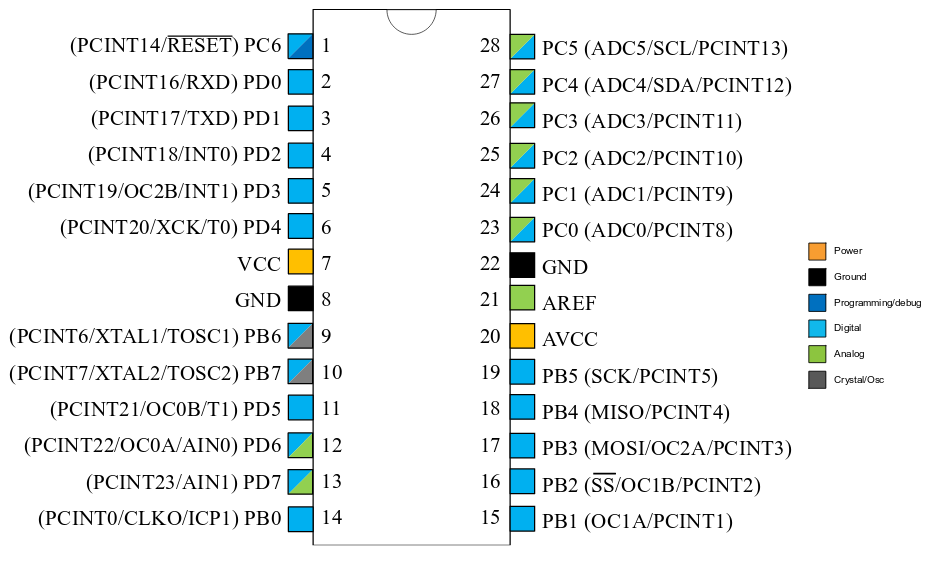
\includegraphics[width=150mm,scale=0.5]{examples/avrpinout}
 \caption{Схема выводов ATMEGA328P-PU}
 \label{avrpinout}
\end{figure}

\newpage

\section{РАЗРАБОТКА УСТРОЙСТВА}

\subsection{Пример ссылки на рисунок}

Я ссылаюсь на рисунок \ref{avrpinout}.

\subsection{Пример таблицы}

\begin{table}[H]
\caption{Предельная толщина препятствия}
\label{penetration}
\begin{tabular}{|l|l|l|}
\hline
\textbf{Частоты} & \textbf{Кирпичная стена, м.} & \textbf{Бетон, м.} \\ \hline
434 МГц & 4.3                 & 0.47      \\ \hline
868 МГц & 2.18                & 0.24      \\ \hline
2.4 ГГц & 0.78                & 0.09      \\ \hline
\end{tabular}
\end{table}

\subsection{Пример нумерованного списка}

\begin{enumerate}
  \item Список доступных устройств для авторизованного;
  \item Кнопка получения дополнительной информации по.
\end{enumerate}

\subsection{Пример ненумерованного списка}

\begin{itemize}
  \item список доступных устройств для авторизованного;
  \item кнопка получения дополнительной информации по.
\end{itemize}

\subsection{Пример ссылки на источник}

Я ссылаюсь на atmelcrystal, описанный в example.bib. \cite{atmelcrystal}

\newpage

\phantomsection
\section*{ЗАКЛЮЧЕНИЕ}
\addcontentsline{toc}{section}{ЗАКЛЮЧЕНИЕ}
% заключение
\newpage

\phantomsection
\renewcommand{\refname}{СПИСОК ИСПОЛЬЗОВАННЫХ ИСТОЧНИКОВ}
\addcontentsline{toc}{section}{СПИСОК ИСПОЛЬЗОВАННЫХ ИСТОЧНИКОВ}
\bibliographystyle{unsrtnat}
\bibliography{example}
\newpage

\phantomsection
\section*{СЛОВАРЬ ТЕРМИНОВ}
\addcontentsline{toc}{section}{СЛОВАРЬ ТЕРМИНОВ}

\begin{itemize}
  \item термин 1: Его значение записывается с заглавной буквы;
  \item термин 2: Его значение записывается с заглавной буквы.
\end{itemize}

\newpage

\begin{landscape}
\phantomsection
\section*{ПРИЛОЖЕНИЕ А}
\addcontentsline{toc}{section}{ПРИЛОЖЕНИЕ А}
\label{appa}

% Пример вставки SVG-изображения (для работы нужен установленный
% inkscape)
%\begin{figure}[H]
% \centering
% \includesvg[width = 700pt]{examples/schematic}
% \caption{Электрическая принципиальная схема разработанного контроллера}
% \label{schematic}
%\end{figure}
\end{landscape}

\phantomsection
\section*{ПРИЛОЖЕНИЕ Б}
\addcontentsline{toc}{section}{ПРИЛОЖЕНИЕ Б}
\label{appb}

\includecode{c}{examples/code.c}{Код приёмопередатчика}

\newpage

\end{document}
